\documentclass{article}
\usepackage{hyperref}
\usepackage{algorithm}
\usepackage{graphicx}
\usepackage{subfig}
 %\usepackage{algorithmic}
 \usepackage{algpseudocode}
\begin{document}
\title{Anti-lost System Documentation}
\author{Li Shitao}
\maketitle
\section{Introduction}

Nowadays, with quick pace of life, people frequently forget or lost their personally things. As the techonology developing significantly, it is naturally to have the idea that the high technology may help people .This anti-lost system is designed and developed to solve this problem using the Bluetooth technology. It can help people quickly find the things that they can not find currently, as well as recording the time and location that the item was last discovered. All the source code is avaliable on  \url{https://github.com/list12356/AntiLost-App.git}.\\
The main functoin and overview of the system is given in Chapter 2, the step of using the system is given in Chapter 3, the details about how the system work will be explained in Chapter 4, and I also gives my future plan in Chapter 5.
\section{Main function}
This system consists of an Android-App and several raspberry-Pi representing the personally things of the user. The main function of this system are listed as following
\begin{itemize}
\item add, remove or edit the device the user want to keep listening
\item quickly send a beep to the device that user want to find within the range of bluetooth communication
\item alarm user when devices are too far from the user
\item record the geographic information once the device is scanned
\end{itemize}
\section{User Guide}
For a new user to use the system, you should keep your bluetooth on in your phone and switch on the raspberry Pi, the Python script will automatically run on the raspberry Pi. Once you finished, open the app, tap the menu in the right-up corner and select the `add item' option, the page will jump to another activity. Press the scan button and youcan get all the bluetooth devices avaliable, select one you want to keep listening and give it a name(blank for its default name). Then you can get the device shown on your main item list. If you no longer want to keep the device, you can select the `delete item` in the menu and choose the device in the delete phrase.
\begin{figure}[htbp]
\subfloat{
\label{fig:3}
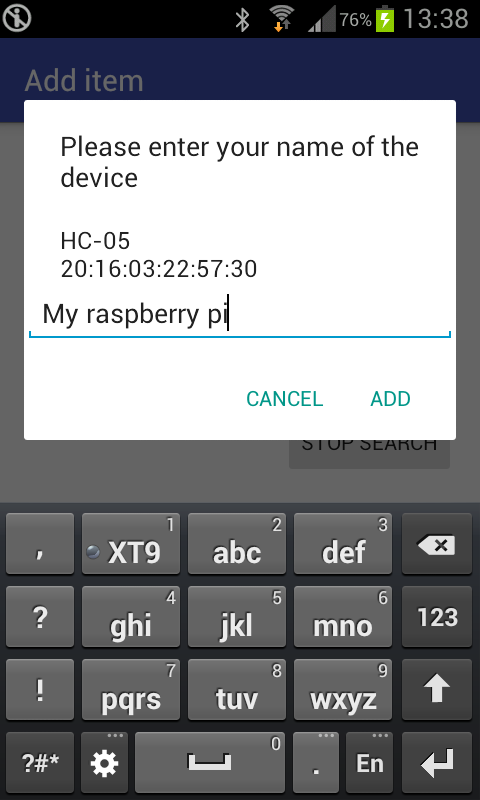
\includegraphics[width =160pt ,keepaspectratio ]{4.png}
}
\subfloat{
\label{fig:4}
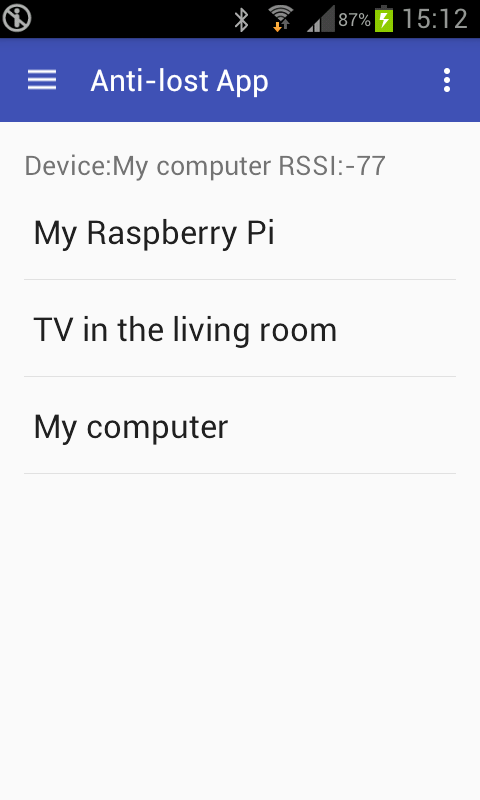
\includegraphics[width =160pt ,keepaspectratio ]{3.png}
}
\end{figure}
\subsection{Find and Call the item}
If you want to find your Item, select it and the program will try to connect it ,if success, you can get the RSSI of the device and a speculated distance according to the RSSI. Choose the `Call my item' button, the program will send a message to the Raspeberry Pi to make it beep. If it fails, you can see the information about the last time and location that the device was scanned. \\
\begin{figure}[t]
\subfloat{
\label{fig:5}
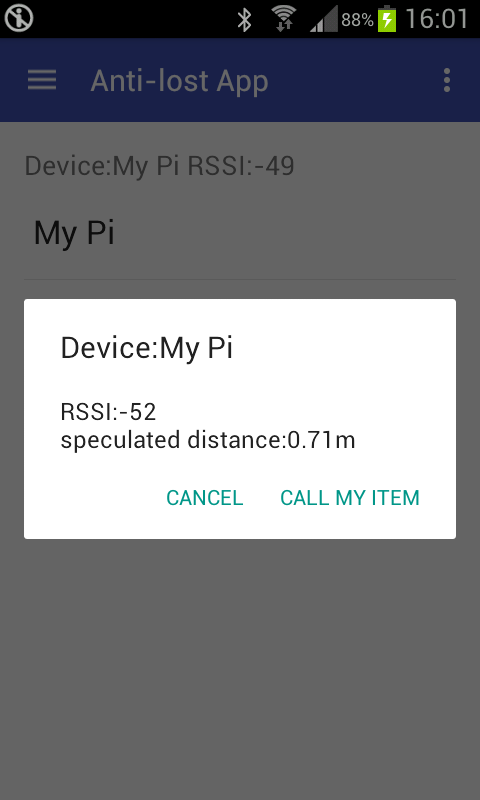
\includegraphics[width =160pt ,keepaspectratio ]{5.png}
}
\subfloat{
\label{fig:6}
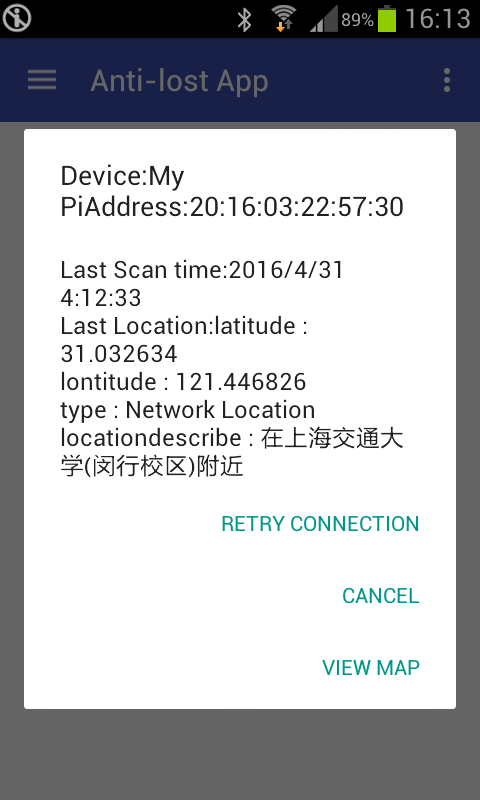
\includegraphics[width =160pt ,keepaspectratio ]{7.png}
}
\end{figure}
If you are too far from your device, the program will auto matically send a message causing both your phone and the Raspberry Pi  to alarm you. Also, whether you want to recieve the alarm and the alarm distance can both be set by the user.
\subsection{User Settings}

\section{Details of impletation}
\subsection{Java Class}
I used two extra java calss to storage the user's information. The first one is the \emph{myItem.java}, it contains the name, address, last scaned time and location of the item. The second one is the \emph{ItemList.java}, it contains a List data stores all the user's items and several methods including add and delete data.
\subsection{The bluetooth communication}
In the MainActivity, there is a timer task run background to scan all the available devices around. Once it discoveres a device that is in the user's item list, it will refresh the information, eg. RSSI, location and time, in the item list. Noticing that the bluetooth discovery will automatically restart in 12 seconds, which is too long a period for the RSSI value to refresh, we set the schedule period of the task to 3 seconds. When user select one item, the program will try to start a connection to the device using a bluetooth socket. The pseudo code is in \ref{alg:Bluetooth}.
May be it is proper to keep the connection in order to save time. However, the bluetooth can only have 8 device connecting at the sametime, and it is a waste of resources considering that in most time there is actually no communication between devices. Besides, in practice, I find that the keeping of connections will influence the quality of the discovery process in some older bluetooth devices. 
\subsection{The location services}
I use the BaiduLocation SDK and BaiduMap SDK to finish the location and map services. In the main activity, there's a listener called \emph{BDLocationListener} to get and recieve the location from the Baidu service. As metioned above, when any device listed in the item list is scaned, its location information will be updated according to this method. In the Map Activity, I use the Baidu Map SDK to draw a map and show the text information
\subsection{The Raspberry Pi}
The model I used is Raspberry Pi Model 2.0B. I used a HC-05 bluetooth adapter and a low-level triggered buzzer. I write a Python program to resolve the message recieved from the HC-05 adapter. The program will read from a FIFO file “/dev/ttyAMA0'' every 0.1s, and once it recieves the message from the FIFO, it will send a high voltage to the GPIO output to beep the buzzer. 
%\section{Experiments}
\section{Conclusion and Future Plan}
The system now just do the basic functions well. In the future, I plan to make an online version. It is intrinsic to think that when every


\end{document}